\chapter{Ordinary Differential Equations II: Boundary Value Problems}\label{ch:ode-boundary}
 
When we solve a Newton equation, a set of initial conditions, i.e.,  initial position $x(t_0)$ and velocity $\dot{x}(t_0)$, are usually specified. In general second order ODEs need two conditions for each variable.  However, a set of initial conditions is not only the way to specify the two independent conditions.  For example, A trajectory $x(t)$ can be uniquely determined by specifying an initial position $x(t_\text{i})$ and a final position $x(t_\text{f})$ (Dirichlet boundary condition). When the two conditions are given at two different time we call it a \emph{boundary value problem}.  It seems strange to use a future position as a condition but it is a popular problem in physics. For example, we could ask a question like how fast we should drive to arrive at the destination in a given time. It is also possible to specify a derivative as a boundary condition (Neumann boundary condition). Boundary value problems are also more common for ODEs with one-dimensional spatial coordinates such as Poisson equation for scalar potential $\varphi(x)$, heat equation for temperature profile $T(x)$, and diffusion equation for particle density $\rho(x)$.   From the numerical view of point, however, there is no difference between temporal and spatial problems.
Eigenvalue problems are also a kind of boundary value problems but we will discuss them in the next chapter.

\section{Shooting method}

In the previous chapter, we solved Newton's equation of motion as an initial value problem.  Now, we solve a Newton equation as a boundary value problem.  Consider the following problem:
The trajectory of a particle of mass $m$ is determined by a Newton's equation of motion
\begin{equation}
\ddot{x} = F(x, \dot{x}, t)
\end{equation}
as before. At time $t=t_\text{i}$, the particle is located at $x_\text{i}$. The particle arrives at $x_\text{f}$ at time $t_\text{f}$.  What are the trajectory $x(t)$ and velocity $v(t)$ of the particle?  This is clearly a boundary value problem.  If we can solve the Newton equation as an initial value problem, the trajectory can be considered as a function of the initial position $x_\text{i}$ and velocity $v_\text{i}$. We write it as $x(t;x_\text{i}, v_\text{i})$.  We know that the particle must be at $x_\text{f}$ at time $t_\text{f}$. Thus, we have $x(t_\text{f}; x_\text{i}, v_\text{i}) = x_\text{f}$ where only $v_\text{i}$ is unknown. By solving this equation for $v_\text{i}$  we find the answer.  This is nothing but a root finding problem.  Once we find the initial velocity, we can find $x(t)$ and $v(t)$ by solving the Newton equation using the method discussed in the previous chapter.  In other words, the boundary value problem is now replaced with an initial value problem combined with root finding.  The root finding method needs a function value $f(v_\text{i}) \equiv  x(t_\text{f}; x_\text{i}, v_\text{i}) - x_\text{f}$.  In other words, we must be able to evaluate $f(v_\text{i})$ for any given $v_\text{i}$.  The evaluation of $f(v_\text{i})$ is an initial value problem and thus we can solve it by the method discussed in the previous chapter.

Since the solution to a Newton equation is unique, there is only one root.  Therefore, the secant method should work well.  Remembering that the secant method needs two initial guesses.  The algorithm known as shooting method is given in Algorithm \ref{algo:shooting}. We shoot again and again not at random but with some intelligence until the target is hit.

\bigskip 
\begin{myalgobox}
    \Algorithm{Shooting method}\label{algo:shooting}
    \medskip
    \begin{minipage}{5.5in}
        \begin{enumerate}
            \item Guess an initial velocity $v_1$.  Here subscript "1" indicates the first try.
            \item Solve the Newton equation as an initial value problem using $v_1$ and get the final position  $x_1=x(t_\text{f})$.  Here the subscript "1" indicates the first try.
            \item If $|x_1 - x_\text{f}| < \text{tolerance}$, we already found a solution. Otherwise continue to step 4.
            \item Change the initial velocity slightly $v_2 = v_1 + \delta$.  This is the second try.
            \item Solve the Newton equation again and get $x_2=x(t_\text{f})$.
            \item If $|x_2 - x_\text{f}| < \text{tolerance}$ then we find a solution.  Otherwise continue step 7.
            \item Now, we enter a loop of the secant method.
            \item $v_{n+1} = v_{n} - \displaystyle\frac{v_{n} - v_{n-1}}{x_{n}-x_{n-1}} \left [ x_n - x_\text{f} \right ]$.  Here, the $(n+1)$-th try is suggested by the secant method.
            \item Solve the Newton equation with $v_{n+1}$ as initial condition and get $x_{n+1} = x(t_\text{f})$.
            \item If $|x_{n+1} - x_\text{f}| < \text{tolerance}$ then we find a solution.  Otherwise repeat from step 8.
        \end{enumerate}
    \end{minipage}
\end{myalgobox}


\bigskip

\medskip
\noindent
\begin{example}[Air Rocket]\label{ex:shoot_rocket}

A compressed air rocket of mass $m=1$ kg is launched vertically from ground.  We want to make it reach height $y_\text{f}=100$ m in $t_\text{f}=2$ s.  At what speed should the rocket be launched?
The Newton equation for the rocket is
\begin{equation}\label{eq:eom_rocket}
m \ddot{y} = - C  |\dot{y}| \dot{y} - m g
\end{equation}
where the\ coefficient\footnote{If only linear drag force is considered the problem is too trivial because we are rooking for a root of a linear equation. The secant method converges immediately at the first iteration.  Quadratic drag force requires at least several steps due to non-linearity.} is $C=0.01$ kg/m. Note that the rocket may reach the desired height at the given time on its way down. 

If the rocket satisfies the condition on its way up, the analytic solution is given by
\begin{equation}
v_\text{i} = \frac{\sqrt{g \lambda} \left [\sqrt{\me^{2 y_\text{f}/\lambda}}-\cos\left (\sqrt{\frac{g\, t_\text{f}^2}{\lambda}}\right )\right ]}{\sin\left (\sqrt{\frac{g\, t_\text{f}^2}{\lambda}}\right )}
\end{equation}
where $\lambda = m/C$.  Substituting all parameter values we obtain $v_\text{i}=101.9281$ m/s.  We try to get this value numerically using the shooting method.  Program \ref{prog:air-rocket} solves the problem using the 4th-order Runge-Kutta and secant methods.  

First, we have to guess the first two steps. The average speed, $50$ m/s, may be a good starting value.  The second guess should be slightly faster since the answer must be larger than the average speed. We use $51$ m/s for the second guess.  Figure \ref{fig:shoot_rocket} shows how the iteration of secant method improves the solution.  Our initial guess is far from the final answer.  Nevertheless the iteration quickly converges to the correct answer. With tolerance $10^{-8}$, the calculation stopped after 6 secant  iterations.  The final velocity is positive and thus the rocket is moving upward.  The final answer $v_\text{i}=101.9968$ m/s is close to the exact one. 

\begin{figure}
\centering
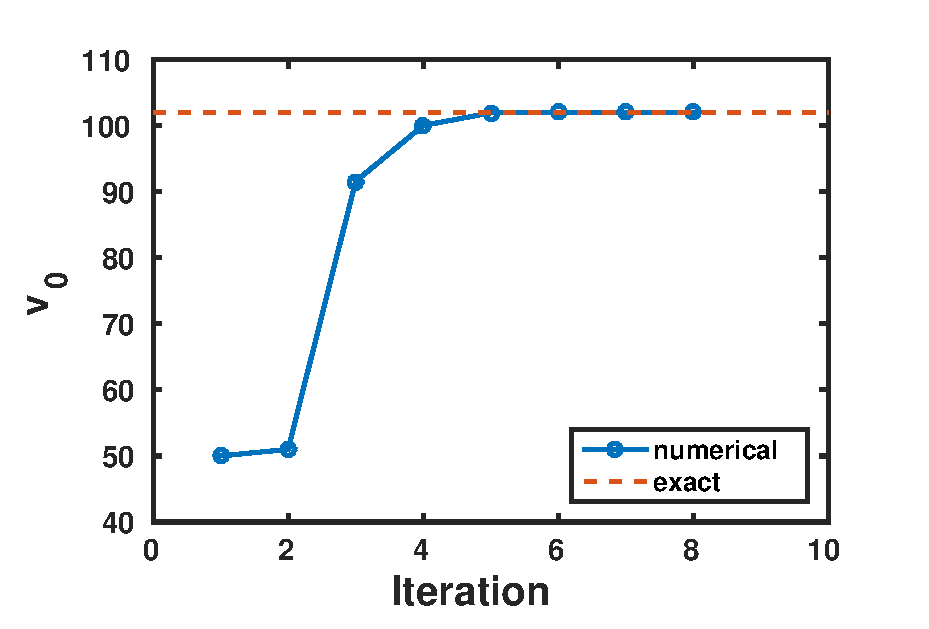
\includegraphics[width=3in]{06.ode2/shoot_rocket.pdf}
\caption{The output of Example \ref{ex:shoot_rocket}. Improvement of the solution as the secant method is iterated.  Initial guesses (step 1 and 2)  are far from the correct answer but the iteration quickly converges to the right answer.}
\label{fig:shoot_rocket}
\end{figure}

\end{example}

\noindent
\section{Numerov method}

An efficient method is availabe for the second-order ODE of the following form:

\begin{equation}
\frac{\md^2 y}{\md x^2} + w(x) y = S(x)
\label{eq:sturm}
\end{equation}
This type of differential equations is popular in physics.  For example, when $w(x)=0$ this equation is equivalent to one-dimensional Poisson equation, heat equation, and diffusion equation.  It becomes a Shr\"{o}dinger equation (energy eigenvalue equation) and Newton equation for parametric harmonic oscillators if $S(x)=0$. 
The algorithm shown below is essentially the same as initial value problems and can be used to solve them.  However, since this type of differential equation appear mostly in boundary value problems, we focus on the boundary value problems. 

Recall the three-points numerical second-order derivative \eqref{eq:diff2-s3},
\begin{equation}
\frac{y_{n+1} - 2 y_n + y_{n-1} }{h^2} = \dv[2]{y}{x} 
+ \frac{h^2}{12} \dv[4]{y}{x} + \order{h^4}
\label{eq:diff2-expansion}
\end{equation}
here we includes the forth order term explicitly.  We can evaluate it  
using the original differential equation as follows:
\begin{eqnarray}
\dv[4]{y}{x} & = & \dv[2]{x} \left( -w(x) y + S(x) \right)\nonumber\\
& = & - \frac{ w_{n+1} y_{n+1} - 2 w_n y_n + w_{n-1} y_{n-1} }
{h^2} + \frac{S_{n+1} - 2 S_n + S_{n-1}} {h^2} + \order{h^2}
\label{eq:diff4}
\end{eqnarray}
where $w_n = w(x_n)$ and $S_n = S(x_n)$.
Substituting Eqs (\ref{eq:diff2-expansion}) and (\ref{eq:diff4}) to Eq (\ref{eq:sturm})
and rearranging $y$'s, the explicit recursive equation is obtained:
\begin{equation}
\begin{split}
\left(1 + \frac{h^2}{12} w_{n+1} \right) y_{n+1}  = &
2 \left( 1 - \frac{5h^2}{12} w_n \right) y_n 
- \left( 1 + \frac{h^2}{12} w_{n-1} \right) y_{n-1} \\
& +  \frac{h^2}{12} \left( S_{n+1} + 10 S_n + S_{n-1} \right) + \order{h^6}
\end{split}
\label{eq:numerov}
\end{equation}
This algorithm is one order more accurate than the fourth-order Runge-Kutta
method and yet $w(x)$ and $S(x)$ are evaluated only one time on the
grid points.  Therefore, the Numerov method is more efficient than
the Runge-Kutta method for this type of the second-order differential
equation.

\bigskip
\begin{example}[One-dimensional Poisson equation]\label{ex:poisson1d}


\begin{figure}
\centering
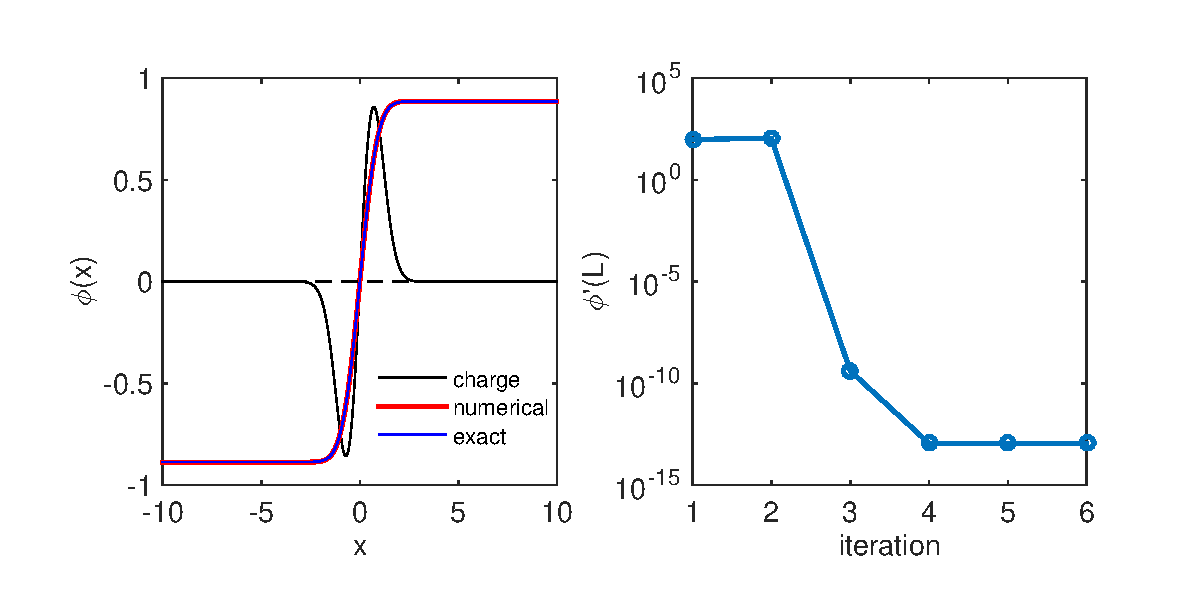
\includegraphics[width=5.5in]{06.ode2/poisson1d.pdf}
\caption{The output of Example \ref{ex:poisson1d}. Left: The profile of the charge density (black), the numerical potential (red) and exact solution (blue). Right: The boundary value of the derivative is iteratively optimized to the correct boundary condition.}
\label{fig:poisson1d}
\end{figure}

\medskip
\noindent
Electric potential $\phi(x)$ in one-dimensional space satisfies the Poisoon equation
\begin{equation}\label{eq:poisson1d}
\phi''(x) = -\frac{\rho(x)}{\epsilon_0}
\end{equation}
where $\rho(x)$ is electric charge density and $\epsilon_0$ vacuum permittivity.  We consider an electric charge density
\begin{equation}\label{eq:charge}
\rho(x) = C x \me^{-x^2}
\end{equation}
where $C$ is a positive constant. The present model has an exact solution 
\begin{equation}
\phi(x) = \frac{\sqrt{\pi}}{2} \erf(x)
\end{equation}
where $\erf$ is the error function. We solve this model numerically using the Numerov method and secant root finding.

For simplicity, we set $C/\epsilon_0=1$.  As Fig. \ref{fig:poisson1d} shows the charge density is localized around $x=0$.
Since $\int_{-\infty}^{\infty} \rho(x) \md x = 0$ (the net charge is zero), the charge is invisible from distance.  Therefore, the potential should be nearly constant at $|x| \gg 1$. Mathematically speaking, the boundary condition is $\displaystyle\lim_{|x| \rightarrow \infty} \phi'(x) = 0$.  This kind of boundary condition at infinity is not suitable for numerical calculation. We assume that $\phi'(\pm L) = 0$ for some large $L$.  A common method integrates the ODE from $x=-L$ using $\phi(-L)$ and $\phi'(-L)$ as boundary conditions.  Since we don't know $\phi(-L)$, we guess one.  Then, we solve the ODE as initial value problem and find $\phi'(L)$.  If this value does not match to the given boundary condition, the initial guess was wrong.  Then, we start over again with a different value of $\phi(-L)$ suggested by the secant method.  

The above method should work well but there is an even better way by taking into account the symmetry of the problem.  Since the charge density is anti-symmetric ($\rho(-x) = -\rho(x)$),  $\phi''(x)$ is also anti-symmetric and thus $\phi(x)$ must be anti-symmetric, too.  Therefore, $\phi(0)=0$.  We can start at $x=0$ and shoot out toward $x=L$. A shorter shooting range is better!  We still have to guess the next function value, $\phi(h)$ where $h$ is step size of $x$. Using $\phi(0)$ and $\phi(h)$, we can find the potential up to the end point $\phi(L)$.  If $|\phi'(L)| < \text{tolerance}$, the guess is correct and we found a solution. Otherwise, repeat the calculation using a new guess suggested by the secant method.  However, we don't know $\phi'(L)$ and thus we need to evaluate it numerically. It does not have to be super accurate and the forward finite difference method \eqref{eq:diff_fwd} is sufficient for this purpose.
\begin{equation}
\phi'(L) = \frac{\phi(L)-\phi(L-h)}{h}
 \end{equation}
In the left panel of Fig \ref{fig:poisson1d}, the numerical solution is compared with the analytic solution. The agreement is so good that they are visually indistinguishable. The right panel shows that the progressive improvement toward the given boundary condition $\phi'(L)=0$.  Despite that the initial guess was quite off the mark, the iteration converges very quickly.
\end{example}

\noindent
\section{Applications in Physics}

\subsection{Quantum Free Falling (See Problem 3.3)}

A quantum particle of mass $m$ is in a uniform gravitational field $g$.  The stationary Schr\"{o}dinger equation is 
\begin{equation}\label{eq:quantum_falling}
\left ( -\frac{\hbar^2}{2m} \frac{\md^2}{\md y^2} + m g y \right ) \psi(y) = E \psi(y)
\end{equation}
where $y$ and $E$ are the position and energy of the particle.  We assume that the particle is dropped from $y=0$ and the gravitational potential energy is also measured from $y=0$.  Under this reference conditions, $E=0$.

Using a normalized coordinate $x=\left( \displaystyle\frac{2 m^2 g}{\hbar^2} \right )^{1/3} y$, Eq. (\ref{eq:quantum_falling}) is simplified to 
\begin{equation}\label{eq:airy}
\frac{\md^2}{\md x^2} \psi(x) = x \psi(x)
\end{equation}
which is known as Airy equation.  Despite of its simple looking, the solution to this equation cannot be expressed in a simple form.  General solution is given by
\begin{equation}
\psi(x) = c_1 \text{Ai}(x) + c_2 \text{Bi}(x)
\end{equation}
where $\text{Ai}(x)$ and $\text{Bi}(x)$ are first and second kind of Airy functions.\cite{airy_function}
Now we apply the first boundary condition.  Since the particle should not be found at $x=\infty$, we impose $\lim_{x \rightarrow \infty} \psi(x) = 0$.  If this is the classical particle, the particle should not move upward.  However, due to uncertainty principle, the quantum particle can be observed slightly above $x=0$.
Since $\displaystyle\lim_{x \rightarrow \infty} \Bi(x) = \infty$, we immediately conclude that $c_2=0$.  What is the second boundary condition?  It turns out that physics imposes no additional condition.\footnote{This is an unbound state and thus we cannot normalize the wave function.}  Hence, $c_1$ can be any finite value.\footnote{It is a convention to set $\text{Ai}(0)=\frac{\Gamma(\frac{2}{3})}{3^{2/3}} = 0.355028\dots$\cite{airy_function}} We could impose a condition such as $\psi(0)=1$ for convenience. It makes the numerical method more time consuming. Therefore, we don't use additional boundary condition and we will utilize this freedom in the numerical method.   

One may try to evaluate the analytical solution.  The integral form of $\text{Ai}(x)$ is given by
\begin{equation}
\Ai(x) = \frac{1}{\pi} \int_0^\infty \cos \left ( \frac{t^3}{3}+x t \right ) \md t\,.
\end{equation}
This integral is \emph{super improper} and none of standard numerical quadrature works.   It is much faster and more accurate to integrate the ODE (\ref{eq:airy}) numerically.  There are other ways to evaluate the Airy functions and many numerical libraries include them. MATLAB has a built-in Airy function \texttt{airy()}.  However, numerical methods to evaluate Airy functions are still actively investigated.\cite{airy_numerical}.

Now, we try to solve the problem by direct numerical integration of the ODE. 
Noting that Eq. (\ref{eq:airy}) is a special case of Eq. (\ref{eq:sturm}) with $w(x)=-x$ and $S(x)=0$, we can integrate it with the Numerov method.  The rigorous boundary condition is $\displaystyle\lim_{x \rightarrow \infty} \psi(x) = 0$ but we replace it with $\psi(x_\text{max})=0, x_\text{max} \gg 1$.  Considering a similar ODE, $y''=y$, has a solution $y \sim \me^{-x}$, we expect $\Ai(x)$ vanishes very quickly, $x_\text{max}=5$ is sufficiently large. 
 In order to use the Numerov method, we need $\psi(x_\text{max}-h)$.
As we discussed above, if $\psi(x)$ is a solution,   $c \psi(x)$ is also a solution and thus we don't have to worry about the magnitude.  This implies that $\psi(x_\text{max}-h)$ can be any finite value. Now we have two points to start the iterations.  At the end, we fix the absolute magnitude by letting $\psi(0)=1$.  This is not a physical condition but just for our convenience.

\begin{figure}
\centering
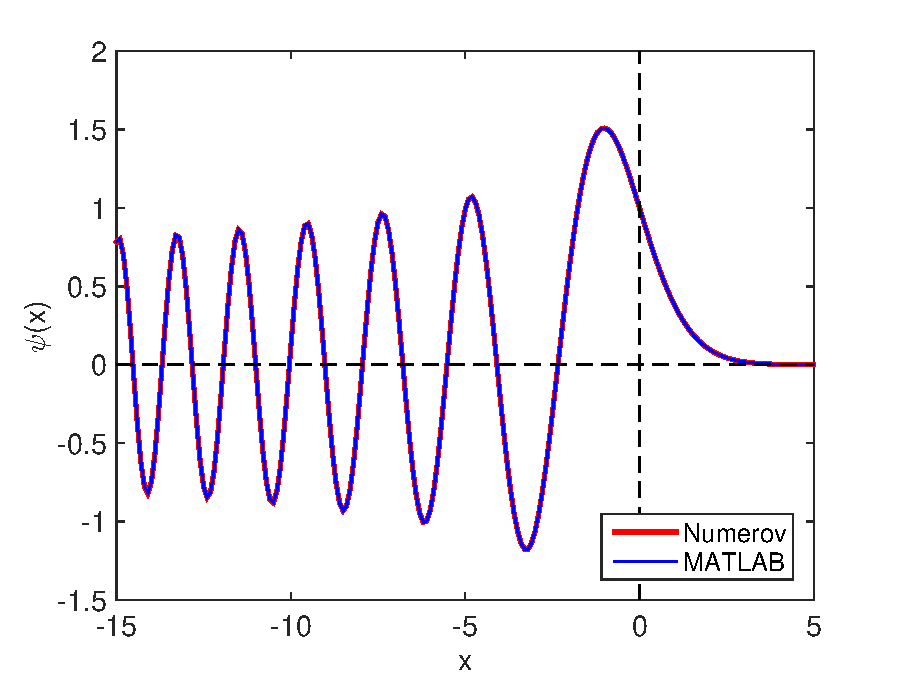
\includegraphics[width=3.0in]{06.ode2/airy_function.pdf}
\caption{The numerical solution (red) to Eq. (\ref{eq:airy}) is compared with the airy function (blue) provided by MATLAB.  Two curves are normalized at $x=0$.}
\label{fig:airy}
\end{figure}

\begin{myalgobox}
    \Algorithm{Airy Equation}
    
    \medskip
    \begin{minipage}{5in}
        \begin{enumerate}
            \item  Starting with $\psi(x_\text{max})=0$ we integrate the equation backward from $x=x_\text{max}$ to $x=x_\text{min}$.
            \item  Choose an integration step $h=-0.1$. (negative because it steps backward.)
            \item  Guess the next value $\psi(x_\text{max}+h)=\delta$.  In principle, we can use any positive value for $\delta$ since the absolute magnitude of the solution cannot be determined until the normalization condition is applied. 
            \item  Integrate the ODE using the Numerov method down to $x_\text{min}$.
            \item  Normalized the solution so that $\psi(0)=1$.
        \end{enumerate}
    \end{minipage}
\end{myalgobox}

Program \ref{prog:qm_free_fall} implements this algorithm.
The results are plotted in MATLAB in Fig. \ref{fig:airy}.  The numerical result agrees well  with the MATLAB built-in airy function.  In the region where the classical particle is prohibited ($x>0$), the wave function decays quickly.  For $x<0$, the wave function oscillates and its wave length decreases as the particle falls down.  Recalling $p=\frac{h}{\lambda}$, as the momentum $p$ increases the wave length $\lambda$ decreases.

 

\subsection{Heating a rod}\label{sec:heating_rod}



A general heat equation for one-dimensional system is given by
\begin{equation}
c_p \rho \frac{\partial T}{\partial t} = \kappa \frac{\partial^2 T}{\partial x^2} + q_\text{loss}
\end{equation}
where $c_p$, $\rho$, and $\kappa$ are specific heat capacity, mass density and heat conductivity, respectively. We also take into account the loss of heat to the environment by $q_\text{loss}$. When the system is in a steady state ($\partial T/\partial t = 0$), this partial differential equation becomes a ODE
\begin{equation}
\kappa \frac{\md^2 T}{\md x^2} = - q_\text{loss}
\end{equation}

Now, we consider a long metallic rod of length $L$ placed in a thermal environment.  The temperature of the environment is kept at $T_0$.
Then, each end of the rod is attached to thermostat so that the temperature of the left end is kept at $T_L>T_0$ and the right end at $T_R >T_0$  As the temperature of the rod is higher than the environment, heat energy dissipate into the environment by
\begin{equation}\label{eq:loss_linear}
q_\text{loss} = - \mu (T(x) - T_0)
\end{equation}
where $\mu$ is a positive constant. This model is valid only when $|T-T_0|$ is small.

Now we calculate the temperature profile of the rod.   It is convenient to use a temperature measured from $T_0$.  Introducing, $u=T-T_0$ and normalized length, $s=x/L$,  the ODE is simplified to
\begin{equation}\label{eq:heating_rod}
\frac{\md ^2}{\md s^2} u(s) = \gamma u(s)
\end{equation}
where $\gamma = \mu L^2/\kappa$ is a dimensionless constant. Letting $w(x)=-\gamma$ and $S(x)=0$, this ODE can be integrated by the Numerov method.


Finally, we want to make it sure that the solution is accurate enough to compute other physical quantities.  As an example, we check the conservation of energy.  In the current setting, energy is injected from the left end of the rod. Its magnitude is determined by the temperature gradient:
\begin{equation}
Q_\text{in} = -\kappa T'(0) \quad \rightarrow \quad - u'(0)
\end{equation}
where the last expression is for dimensionless calculation.  Similarly energy loss from the right end is
\begin{equation}
Q_\text{out} = +\kappa T'(L)\quad \rightarrow \quad + u'(1) 
\end{equation}
and the heat dissipation through the surface of the rod is given by
\begin{equation}
Q_\text{diss} = - \mu \int_0^L [T(x)-T_0] \md x \quad \rightarrow \quad - \gamma \int_0^1 u(s) \md s
\end{equation}
Since the net energy transaction must be balanced, $Q_\text{in}+Q_\text{out}+Q_\text{diss} =0$.  

Program \ref{prog:heating_rod} calculates the temperature profile using the Numerov method and evaluates the energy transaction. Now, pick parameter values.  All constants ($\mu, L, \kappa$) are combined together into one parameter $\gamma$ and thus we don't have to specify each parameter value.  We use $\gamma=10$ in the example calculation.   The example boundary conditions are $u(0)=1$ and $u(1)=0$. It is not necessary to compute other value of $u(0)$ because eq. (\ref{eq:heating_rod}) is linear.  If $u(x)$ is a solution, $c\, u(x)$ is also a solution.  If you change the temperature at the left end as $T_L=100$, the solution would be $100 u(x)$. There is no need to recalculate the solution.
If the heat loss is not linear to the temperature difference, we cannot use this trick. (See Problem 5.1.) 

The temperature profile is plotted in the left panel of Fig \ref{fig:heating_rod}. When the temperature is high, heat dissipation is faster and thus temperature gradient is larger near the left edge. If the heat dissipation to the environment is not considered, the profile is a straight line from $T_L$ to $T_R$. The effect of the dissipation is clearly visible in the plot. The right panel shows the error after each iteration. The improvement is not very fast but steady.  Here is the output of the energy transaction:

\begin{center}

\begin{minipage}{0.85\textwidth}
\small
\begin{Verbatim}[frame=single]
Q_in=3.173136,  Q_out=-3.129448,  Q_diss=-0.043694,  Q_net=-0.000007
\end{Verbatim}
\end{minipage}
\end{center}
The energy conserves with 5 significant figures.  

\begin{figure}
\centering
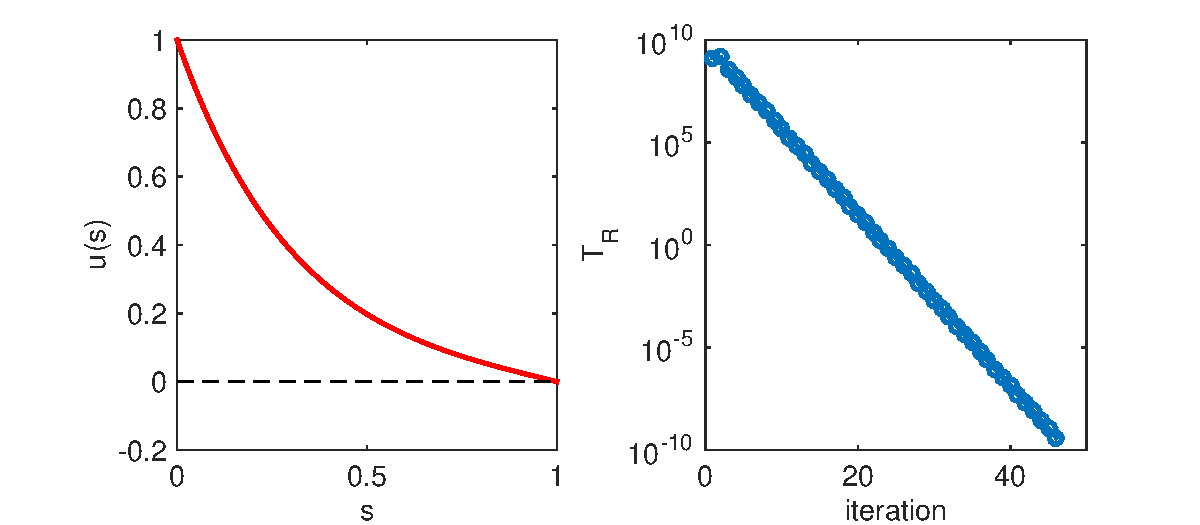
\includegraphics[width=5in]{06.ode2/heating_rod.pdf}
\caption{Left: The numerical solution to Eq. (\ref{eq:heating_rod}). Right: Error after each secant iteration.}
\label{fig:heating_rod}
\end{figure}





\newpage
\noindent
\section{Problems}

\begin{enumerate}[labelwidth=0.5cm,labelindent=0cm,leftmargin=*,label=\bfseries \thechapter.\arabic*,align=left]

\item \textbf{Heating Rod with Nonliear Heat Loss}

In Sec \ref{sec:heating_rod}, the temperature profile is computed with  the linear heat loss (\ref{eq:loss_linear}) which is valid only when the temperature is not far from the temperature of the environment.  When temperature difference becomes large,  heat loss due to radiation becomes dominant.  In that case, the loss density is given by
\begin{equation}
q_\text{loss} = - \mu (T^4 - T_0^4)
\end{equation}
Find the temperature profile.  Note that the Numerov method cannot be used with this loss function. Use the 4th-order Rung-Kutta instead.

\item \textbf{Cannon}

\medskip
\noindent
A cannon ball is shot at a target located $1200$ m away on the same level of ground.  The initial speed of the cannon ball is fixed to $v_0=150$ m/s. You can control only the elevation angle $\theta$.  Taking into account quadratic friction, the equation of motion is given by
\begin{equation}\label{eq:projectile_quad_drag}
m \frac{\md^2}{\md t^2} \vec{v} = - b v \vec{v} - m g \hat{z}
\end{equation}
where $v$ is the magnitude of the velocity $\vec{v}$ and $\hat{z}$ is a unit vector in the vertical upward direction.  The coefficient $b$ is defined by 
\begin{equation}
b=\frac{1}{2} \rho C_D A
\end{equation}
where $\rho$ is the mass density of air, $C_D$ dimensionless drag coefficient, and $A$ is the cross sectional area of the cannon ball.  Reasonable parameter values are $m=5$ kg, $A=9 \times 10^{-3}$ m$^2$, $\rho=1.2$ kg/m$^3$, $C_D=0.5$. At what angle $\theta$ the target is hit?
\end{enumerate}


\newpage
\section*{MATLAB Source Codes}
\addcontentsline{toc}{section}{\protect\numberline{}MATLAB Source Codes}

\bigskip
\noindent
\program
\label{prog:air-rocket}

\footnotesize
\begin{verbatim}
%**************************************************************************
%*     Example  6.1                                                       *
%*     filename: ch06pr01.m                                               *
%*     program listing number: 6.1-1                                      *
%*                                                                        *
%*     This program determines a launching speed that a rocket necessary  *
%*     to reach height yf in travel time tf.                              *
%*     Use function: rocket_trajectory(v,t)                               *
%*                                                                        *
%*     Programed by Ryoichi Kawai for Computational Physics Course.       *
%*     Last modification:  10/13/2013.                                    *
%**************************************************************************
clear all;

% set the boundary conditions
yf=100; tf=2;

% tolerance
tol=1e-8;

% control variable 
found = false;

% first guess
n=1;
v(n) = 50;
[y(n), vf] = rocket_trajectory(v(n),tf);
if abs(y(n)-yf) < tol
    found = true;
    v0 = v(n);
end

%second guess
n=n+1;
v(n) = 51;
[y(n), vf] = rocket_trajectory(v(n),tf);
if abs(y(n)-yf) < tol
    found = true;
    v0 = v(n);
end

% secant iteration
while not(found)
    v(n+1) = v(n) - (v(n)-v(n-1))/(y(n)-y(n-1))*(y(n)-yf);
    [y(n+1), vf] = rocket_trajectory(v(n+1),tf);
    if abs(y(n+1)-yf) < tol
       found = true;
       v0 = v(n+1);
    end
    n=n+1;
end

% show the result
fprintf('initial velocity = %.6f final velocity = %.6f \n',v(n),vf)

% plot the convergency
p=plot([1:n],v,'-o',[0,n+2],[101.9281,101.9281],'--');
xlabel('Iteration','Fontsize',14)
ylabel(texlabel('v_0'),'Fontsize',14)
axis([0 n+2 40 110])
set(p(1),'linewidth',2)
legend('numerical','exact')
legend('location','southeast')
\end{verbatim}

\begin{verbatim}
%**************************************************************************
%*     Example  6.1                                                       *
%*     filename: rocket_trajectory.m                                      *
%*     program listing number: 6.1-2                                      *
%*     Called by ch06pr01.m                                               *
%*                                                                        *
%*     This function detemines the trajectory of the rocket for a given   *
%*     initial velocity and the final time.                               *
%*        Input:  vi = initial velocity                                   *
%*                 t = final time                                         *
%*        Output:  y = final position of the rocket                       *
%*                 v = final velocity of the rocket                       *
%*                                                                        *
%*     Programed by Ryoichi Kawai for Computational Physics Course.       *
%*     Last modification:  10/13/2013.                                    *
%**************************************************************************
function [y,v]=rocket_trajectory(vi,t)

% This function calculat the height of the rocket at t;
% system parameter values
g=9.8; m=1;  C=0.01;

% control parameters
N=1000;
h=t/N;

% define force/mass as a function of v
f=@(v) -(C/m)*abs(v)*v-g;

% initial conditions
y0=0;
v0=vi;

% 4th-order Runge-Kutta
for n=1:N-1
    ky1 = v0;
    kv1 = f(v0);

    y_mid = y0 + ky1*h/2;
    v_mid = v0 + kv1*h/2;
    ky2 = v_mid;
    kv2 = f(v_mid);
      
    y_mid = y0 + ky2*h/2;
    v_mid = v0 + kv2*h/2;
    ky3 = v_mid;
    kv3 = f(v_mid);

    y_end = y0 + ky3*h;
    v_end = v0 + kv3*h;
    ky4 = v_end;
    kv4 = f(v_end);
    
    y0=y0+(ky1+2*(ky2+ky3)+ky4)*h/6;
    v0=v0+(kv1+2*(kv2+kv3)+kv4)*h/6;
end

% return the final height and velocity
y=y0;
v=v0;
end
\end{verbatim}
\normalsize

\ruleend

\bigskip
\noindent
\program
\label{prog:poisson1d}

\footnotesize
\begin{verbatim}
%**************************************************************************
%*     Example  6.2                                                       *
%*     filename: ch06pr02.m                                               *
%*     program listing number: 6.2-1                                      *
%*                                                                        *
%*     This program solves one-dimensional Poisson equation using         *
%*     Numerov integration and secant root finding methods.               *
%*     Use function: numerov_poisson(y,L)                                 *
%*                                                                        *
%*     Programed by Ryoichi Kawai for Computational Physics Course.       *
%*     Last modification:  10/13/2013.                                    *
%**************************************************************************
clear all;

% set the boundary conditions
L=10;
% tolerance
tol=1e-16';
% control variable 
found = false;

n=1;
% first guess of phi_1
y1(n) = 0.1;
% get the potential phi(x)
y = numerov_poisson(y1(n),L);
N = size(y,1);   % check how many grid points are used.
% derivative of phi(x) at the end point.
y2(n) = (y(N,2)-y(N-1,2))/(y(N,1)-y(N-1,1));
if abs(y2(n)) < tol
    found = true;
end

if not(found)
    n=n+1;
    % second guess of phi_1
    y1(n) = y1(n-1)+0.01;
    % get the potential phi(x)
    y = numerov_poisson(y1(n),L);
    % derivative of phi(x) at the end point.
    y2(n) = (y(N,2)-y(N-1,2))/(y(N,1)-y(N-1,1));
    if abs(y2(n)) < tol
         found = true;
    end
end

% secant iteration
while not(found)
    % guess phi_1 by secant method
    y1(n+1) = y1(n) - (y1(n)-y1(n-1))/(y2(n)-y2(n-1))*y2(n);
    % derivative of phi(x) at the end point.
    y = numerov_poisson(y1(n+1),L);
     % derivative of phi(x) at the end point.
    y2(n+1) = (y(N,2)-y(N-1,2))/(y(N,1)-y(N-1,1));
    if abs(y2(n+1)) < tol
         found = true;
    end
    n=n+1;
end

% construct the whole curve from x=-L to x=L.
X(1:N) = -y(N:-1:1,1); X(N+1:2*N)=y(1:N,1);
Y(1:N) = -y(N:-1:1,2); Y(N+1:2*N)=y(1:N,2);

%plot charge density
subplot(1,2,1)
p1=plot(X,2.*X.*exp(-X.*X));
set(p1,'color','black')
hold on
% plot the numerical potential
p2=plot(X,Y);
set(p2,'Linewidth',2,'color','red')
xlabel('x','fontsize',14)
ylabel(texlabel('phi(x)'),'fontsize',14)
axis([-L L -1 1])
hold on
% plot the analytic potential
p3=plot(X,sqrt(pi)/2*erf(X));
set(p3,'color','blue')
legend('charge','numerical','exact')
legend('Location','southeast')
hold on
% plot the zero line
p4=plot([-L,L],[0,0],'--');
set(p4,'color','black')
hold off

subplot(1,2,2)
% plot the improvment of the first point.
q=semilogy([1:n],abs(y2),'-o');
xlabel('iteration')
ylabel(texlabel('phi''(L)'))
%axis([0 8 0.0001 1])
set(q,'linewidth',2)
\end{verbatim}

\bigskip
\begin{verbatim}
%**************************************************************************
%*     Example  6.2                                                       *
%*     filename: numerov_poisson.m                                        *
%*     program listing number: 6.2-2                                      *
%*     Called by ch06pr02.m                                               *
%*                                                                        *
%*     This function integrates a one-dimensional Poisson equation for    *
%*     given initial velocity and the final time.                         *
%*        Input:  y1 = y(h)                                               *
%*                 L = boundary                                           *
%*        Output:  y = y(L)                                               *
%*                                                                        *
%*     Programed by Ryoichi Kawai for Computational Physics Course.       *
%*     Last modification:  10/13/2013.                                    *
%**************************************************************************
function [y]=numerov_poisson(y1,L)

% control parameters
N=10000; h=L/N;
y=zeros(N+1,2);  % y(:,1) is position x
                 % y(:,2) is field phi(x)

% define S(x) in Numerov method
S=@(x) -2*x*exp(-x^2);

% initial conditions
% due to symmetry phi(0)=0
n=1;
y(n,1)=0;
y(n,2)=0;
s(n)=S(y(n,1));

% we guess phi(h)=phi_1
n=n+1;
x(n,1)=y(n-1,1)+h;
y(n,2)=y1;
s(n)=S(y(n,1));

% shoot out to x=L by the Numerov method
for n=2:N
  y(n+1,1) = y(1,1) + (n-1)*h;
  s(n+1)=S(y(n+1,1));
  y(n+1,2) = 2*y(n,2)-y(n-1,2)+(s(n+1)+10*s(n)+s(n-1))*h^2/12;
end

end
\end{verbatim}

\normalsize

\ruleend
\bigskip
\noindent
\program
\label{prog:qm_free_fall}

\footnotesize
\begin{verbatim}
%**************************************************************************
%*     Section  6.3.1                                                     *
%*     filename: ch06pr03.m                                               *
%*     program listing number: 6.3                                        *
%*                                                                        *
%*     This program finds the wave function of freely falling particle.   *
%*     to reach height yf in travel time tf.                              *
%*                                                                        *
%*     Programed by Ryoichi Kawai for Computational Physics Course.       *
%*     Last modification:  10/13/2013.                                    *
%**************************************************************************
clear all;
clc

% control parameters
xmax = 5;
xmin = -15;

% Integrating from xmax to 0

h = -0.1;
N = ceil((xmin-xmax)/h);

% define w(x) in Numerov method
W = @(x) -x;

% initial conditions
n = 1;
y(n,1) = xmax;
y(n,2) = 0;
w(n) = W(y(n,1));

% we guess next value
n = n+1;
y(n,1) = y(n-1,1)+h;
y(n,2) = y(n-1,2)+0.1;
w(n) = W(y(n,1));

% shoot left by the Numerov method
for n=2:N
  y(n+1,1) = y(n,1) + h;
  w(n+1) = W(y(n+1,1));
  y(n+1,2) = 2*(1-5*h^2*w(n)/12)*y(n,2) - (1+h^2*w(n-1)/12)*y(n-1,2); 
  y(n+1,2) = y(n+1,2)/(1+h^2*w(n+1)/12);
end

% normalization
N0 = int32(-xmax/h)+1; % find the location of x=0
y(:,2) = y(:,2)/y(N0,2);


p=plot(y(:,1),y(:,2),y(:,1),airy(y(:,1))/airy(0));
xlabel('x')
ylabel(texlabel('psi(x)'))
set(p(1),'linewidth',2,'color','red');
set(p(2),'linewidth',1,'color','blue');
legend('Numerov','MATLAB');
legend('location','southeast');
hold on
q=plot([-15, 5],[0,0],'--',[0,0],[-1.5,2],'--');
set(q,'color','black');
axis([-15 5 -1.5 2]);
hold off
\end{verbatim}
\normalsize

\ruleend
\bigskip
\noindent
\program
\label{prog:heating_rod}

\footnotesize
\begin{verbatim}
%**************************************************************************
%*     Section 6.3.2                                                       *
%*     filename: ch06pr04.m                                               *
%*     program listing number: 6.4-1                                      *
%*                                                                        *
%*     This program solves one-dimensional heat equation and finds        *
%*     temperature profile and heat energy transaction using              *
%*     Numerov integration.                                               *
%*     Use function: numerov_heat(TL,delta,L)                             *
%*                                                                        *
%*     Programed by Ryoichi Kawai for Computational Physics Course.       *
%*     Last modification:  10/13/2013.                                    *
%**************************************************************************

clear all;
% system parameters
global mu
mu = -10;
TL=1;  TR=0; L=1;
% tolerance
tol=1e-9;
% control variable 
found = false;

n=1;
% first guess of delta
y1(n) = 1;
% get the u(x)
y = numerov_heat(TL,y1(n),L);
N = size(y,1);   % check how many grid points are used.
y2(n)=(y(N,2)-TR)^2;
if abs(y2(n)) < tol
    found = true;
end

if not(found)
    n=n+1;
    % second guess of delta
    y1(n) = y1(n-1)+0.01;
    % get u(x)
    y = numerov_heat(TL,y1(n),L);
    y2(n)=(y(N,2)-TR)^2;
    if abs(y2(n)) < tol
         found = true;
    end
end

% secant iteration
while not(found)
    % guess delta by secant method
    y1(n+1) = y1(n) - (y1(n)-y1(n-1))/(y2(n)-y2(n-1))*y2(n);
    % derivative of phi(x) at the end point.
    y = numerov_heat(TL,y1(n+1),L);
    y2(n+1)=(y(N,2)-TR)^2;
    if abs(y2(n+1)) < tol
        found = true;
    end
    n=n+1;
end

% Energy conservation
Q_in = -(y(2,2)-y(1,2))/(y(2,1)-y(1,1));
Q_out= +(y(n,2)-y(n-1,2))/(y(n,1)-y(n-1,1));
Q_diss = mu*sum(y(1:2:n-2,2)+4*y(2:2:n-1,2)+y(3:2:n,2))*(y(2,1)-y(1,1))/3;
fprintf('Q_in=%.6f,  Q_out=%.6f,  Q_diss=%.6f,  Q_net=%.6f\n',...
    Q_in, Q_out, Q_diss, Q_in+Q_out+Q_diss);

% plot heat source
subplot(1,2,1)
p=plot(y(:,1),y(:,2));
set(p,'Linewidth',2,'color','red')
xlabel('s','fontsize',14)
ylabel(texlabel('u(s)'),'fontsize',14)
hold on

p2=plot([0,L],[0,0],'--');
set(p2,'color','black')
hold off

subplot(1,2,2)
% plot the error after each iteration.
q=semilogy([1:n],abs(y2),'-o');
xlabel('iteration','fontsize',14)
ylabel(texlabel('T_R'),'fontsize',14)
set(q,'linewidth',2)
\end{verbatim}

\bigskip
\begin{verbatim}
%**************************************************************************
%*     Section 6.3.2                                                      *
%*     filename: numerov_heat.m                                           *
%*     program listing number: 6.3-2                                      *
%*     Called by ch06pr02.m                                               *
%*                                                                        *
%*     This function integrates a one-dimensional heat equation.          *
%*        Input:  TL = temperature at the left end of the rod             *
%*             delta = decrease of the temperature at next point          *
%*                 L = length of the rod                                  *
%*        Output:  y = position y(:,1) and temperature profile y(:,2)     *
%*                                                                        *
%*     Programed by Ryoichi Kawai for Computational Physics Course.       *
%*     Last modification:  10/13/2013.                                    *
%**************************************************************************
function [y]=numerov_heat(TL,delta,L)

global mu

% control parameters
N=10000; h=L/N;
y=zeros(N+1,2);  % y(:,1) is position x
                 % y(:,2) is field u(x)

% define w(x) in Numerov method
w=mu;

% initial conditions
n=1;
y(n,1)=0;
y(n,2)=TL;

% we guess u(h)
n=n+1;
y(n,1)=y(n-1,1)+h;
y(n,2)=y(n-1,2)-delta;

% shoot out to x=L by the Numerov method
for n=2:N
  y(n+1,1) = y(1,1) + (n-1)*h;
  y(n+1,2) = 2*(1-5*h^2*w/12)*y(n,2) - (1+h^2*w/12)*y(n-1,2);
  y(n+1,2) = y(n+1,2)/(1+h^2*w/12);
end

end
\end{verbatim}
\normalsize

\bigskip
\noindent
\section*{Python Source Codes}
\addcontentsline{toc}{section}{\protect\numberline{}Python Source Codes}
\setcounter{program}{0}

\bigskip
\noindent
\program
\footnotesize
\begin{verbatim}
#!/usr/bin/env python3
# -*- coding: utf-8 -*-
"""
%**************************************************************************
%*     Example  6.1                                                       *
%*     filename: ch06pr01.py                                              *
%*     program listing number: 6.1-1                                      *
%*                                                                        *
%*     This program determines a launching speed that a rocket necessary  *
%*     to reach height yf in travel time tf.                              *
%*                                                                        *
%*     Programed by Ryoichi Kawai for Computational Physics Course.       *
%*     Last modification:  10/13/2013.                                    *
%**************************************************************************
"""
import numpy as np
import matplotlib.pyplot as plt

def f(v):
    # right hand side of the ODE
    g=9.8; m=1.0; C=0.01
    return -(C/m)*np.abs(v)*v-g

def rocket_trajectory(vi,t):
    # Solve the ODE using RK5 and return the final position abd velocity
    N=1000
    h=t/N
    y0=0.0
    v0=vi
    
    for n in range(N):
        ky1 = v0
        kv1 = f(v0)

        y_mid = y0 + ky1*h/2.0
        v_mid = v0 + kv1*h/2.0
        ky2 = v_mid
        kv2 = f(v_mid)
      
        y_mid = y0 + ky2*h/2.0
        v_mid = v0 + kv2*h/2.0
        ky3 = v_mid
        kv3 = f(v_mid)

        y_end = y0 + ky3*h
        v_end = v0 + kv3*h
        ky4 = v_end
        kv4 = f(v_end)
    
        y0=y0+(ky1+2*(ky2+ky3)+ky4)*h/6.0
        v0=v0+(kv1+2*(kv2+kv3)+kv4)*h/6.0

    return [y0,v0]

if __name__ == "__main__":
    # set the boundary conditions
    yf=100.0; tf=2.0

    # tolerance
    tol=1e-8

    # control variable 
    nmax = 100
    found = False

    y=np.zeros(nmax+1)
    v=np.zeros(nmax+1)
    # first guess
    n=1
    v[n] = 50.0
    [y[n], vf] = rocket_trajectory(v[n],tf)
    if np.abs(y[n]-yf) < tol :
        found = True
        v0 = v[n]

    #second guess
    n+=1
    v[n] = 51.0
    [y[n], vf] = rocket_trajectory(v[n],tf)
    if np.abs(y[n]-yf) < tol:
        found = True
        v0 = v[n]

# secant iteration
    while not(found) :
        v[n+1] = v[n] - (v[n]-v[n-1])/(y[n]-y[n-1])*(y[n]-yf)
        [y[n+1], vf] = rocket_trajectory(v[n+1],tf)
        if np.abs(y[n+1]-yf) < tol:
            found = True
            v0 = v[n+1]
        n+=1

    # show the result
    print('initial velocity = {0:10.6f} final velocity = {1:10.6f}'
          .format(v[n],vf))

    # plot the convergency
    plt.ioff()
    plt.figure(figsize=(6,5))
    plt.plot(np.linspace(1,n,n),v[1:n+1],'-ob',label='numerical')
    plt.plot([0,n+2],[101.9281,101.9281],'--',label='exact')
    plt.xlabel('Iteration')
    plt.ylabel('$v_0$')
    plt.legend(loc=4)
    plt.show()
\end{verbatim}
\normalsize

\bigskip
\noindent
\program
\footnotesize
\begin{verbatim}
#!/usr/bin/env python3
# -*- coding: utf-8 -*-
"""
%**************************************************************************
%*     Example  6.2                                                       *
%*     filename: ch06pr02.py                                              *
%*     program listing number: 6.2-1                                      *
%*                                                                        *
%*     This program solves one-dimensional Poisson equation using         *
%*     Numerov integration and secant root finding methods.               *
%*     Use function: numerov_poisson(y,L)                                 *
%*                                                                        *
%*     Programed by Ryoichi Kawai for Computational Physics Course.       *
%*     Last modification:  10/13/2013.                                    *
%**************************************************************************
"""
import numpy as np
import matplotlib.pyplot as plt
from scipy.special import erf

def S(x):
    return -2.0*x*np.exp(-x**2)
    
def numerov_poisson(y1,L,N):
#    control parameters
    h=L/N
    x=np.linspace(0,L,N+1)
    y=np.zeros(N+1)  # field phi(x)
    s=np.zeros(N+1)

    # initial conditions
    # due to symmetry phi(0)=0
    y[0]=0.0
    s[0]=S(y[0])

    # we guess phi(h)=phi_1
    y[1]=y1
    s[1]=S(x[1])

    # shoot out to x=L by the Numerov method
    n=1
    while n < N :
        s[n+1]=S(x[n+1])
        y[n+1] = 2.0*y[n]-y[n-1]+(s[n+1]+10.0*s[n]+s[n-1])*h**2/12.0
        n+=1
        
    return x, y

if __name__ == "__main__":
    # set the boundary conditions
    L=10.0
    N=10000
    # tolerance
    tol=1.0e-16
    # control variable 
    found = False

    y1=np.zeros(101)
    y2=np.zeros(101)
    n=1
    # first guess of phi_1
    y1[0] = 0.1

    # get the potential phi(x)
    x, y = numerov_poisson(y1[0],L,N)

    # derivative of phi(x) at the end point.
    y2[0] = (y[N]-y[N-1])/(x[N]-x[N-1])
    if np.abs(y2[0]) < tol:
        found = True

    if not(found):
        # second guess of phi_1
        y1[1] = y1[0]+0.01
        # get the potential phi(x)
        x, y = numerov_poisson(y1[1],L,N)
        # derivative of phi(x) at the end point.
        y2[1] = (y[N]-y[N-1])/(x[N]-x[N-1])
        if np.abs(y2[1]) < tol:
                  found = True

    # secant iteration
    n=1
    while not(found):

        # guess phi_1 by secant method
        y1[n+1] = y1[n] - (y1[n]-y1[n-1])/(y2[n]-y2[n-1])*y2[n]
        # derivative of phi(x) at the end point.
        x, y = numerov_poisson(y1[n+1],L,N)
        # derivative of phi(x) at the end point.

        y2[n+1] = (y[N]-y[N-1])/(x[N]-x[N-1])
        if np.abs(y2[n+1]) < tol:
            found = True

        n+=1
        print("Itertation ={0:5d}, y2={1:15.5e}".format(n,y2[n]))

    # construct the whole curve from x=-L to x=L.
    X=np.zeros(2*N+1)
    Y=np.zeros(2*N+1)
    X[0:N] = -x[N:0:-1]; X[N:2*N+1]=x[0:N+1]
    Y[0:N] = -y[N:0:-1]; Y[N:2*N+1]=y[0:N+1]

    #plot charge density
    plt.ioff()
    plt.figure(figsize=(12,5))
    plt.subplot(1,2,1)
    plt.plot(X,2*X*np.exp(-X*X),'-g',label=r"$\rho(x)$")

    # plot the numerical potential
    plt.plot(X,Y,'-r',linewidth=2.0,label="Numerical")
    # plot the analytic potential
    plt.plot(X,np.sqrt(np.pi)/2.0*erf(X),'-b',label="Exact")
    plt.plot([-L,L],[0.0,0.0],'--k')
    plt.xlabel('x')
    plt.ylabel(r"$\phi(x)$")
    plt.legend(loc=4)

    plt.subplot(1,2,2)
    # plot the improvment of the first point.
    plt.semilogy(np.linspace(0,n,n+1),abs(y2[0:n+1]),'-o')
    plt.xlabel('iteration')
    plt.ylabel("$\phi'(L)$")
    plt.show()
\end{verbatim}
\normalsize
\bigskip
\noindent
\program
\footnotesize
\begin{verbatim}
#!/usr/bin/env python3
# -*- coding: utf-8 -*-
"""
%**************************************************************************
%*     Section  6.3.1                                                     *
%*     filename: ch06pr03.py                                              *
%*     program listing number: 6.3                                        *
%*                                                                        *
%*     This program finds the wave function of freely falling particle.   *
%*     to reach height yf in travel time tf.                              *
%*                                                                        *
%*     Programed by Ryoichi Kawai for Computational Physics Course.       *
%*     Last modification:  10/13/2013.                                    *
%**************************************************************************
"""
import numpy as np
import matplotlib.pyplot as plt
from scipy.special import airy 

# define w(x) in Numerov method
def W(x):
    return -x

# control parameters
xmax = 5.0
xmin = -15.0

# Integrating from xmax to 0
N = 200
h = (xmin-xmax)/np.float(N)
x = np.linspace(xmax,xmin,N+1)
y = np.zeros(N+1)
w = np.zeros(N+1)

# initial conditions
y[0] = 0
w[0] = W(x[0])

# we guess next value
y[1] = y[0]+0.1
w[1] = W(x[1]);

# shoot left by the Numerov method
for n in range(1,N):
  w[n+1] = W(x[n+1]);
  y[n+1] = 2.0*(1.0-5.0*h**2*w[n]/12.0)*y[n] - (1.0+h**2*w[n-1]/12.0)*y[n-1]
  y[n+1] = y[n+1]/(1.0+h**2*w[n+1]/12.0)

# normalization
N0 = np.int(-xmax/h) # find the location of x=0
y[:] = y[:]/y[N0]


plt.figure(figsize=(6,5))
plt.plot(x,y,'-r',label="Numerov",linewidth=2.5)
plt.plot(x,airy(x)[0]/airy(0)[0],'-b',label="Exact")
plt.xlabel('x')
plt.ylabel(r'$\psi(x)$')
plt.legend(loc=4)
plt.plot([-15, 5],[0,0],'--k',[0,0],[-1.5,2],'--k')
plt.show()
\end{verbatim}
\normalsize
\bigskip
\noindent
\program
\footnotesize
\begin{verbatim}
#!/usr/bin/env python3
# -*- coding: utf-8 -*-
"""
%**************************************************************************
%*     Section 6.3.2                                                      *
%*     filename: ch06pr04.py                                              *
%*     program listing number: 6.4-1                                      *
%*                                                                        *
%*     This program solves one-dimensional heat equation and finds        *
%*     temperature profile and heat energy transaction using              *
%*     Numerov integration.                                               *
%*     Use function: numerov_heat(TL,delta,L)                             *
%*                                                                        *
%*     Programed by Ryoichi Kawai for Computational Physics Course.       *
%*     Last modification:  10/13/2013.                                    *
%**************************************************************************
"""
import numpy as np
import matplotlib.pyplot as plt

def numerov_heat(TL,delta,L):
    global mu
    # control parameters
    N=10000; h=L/N
    x=np.linspace(0,L,N+1)
    u=np.zeros(N+1)

    # define w(x) in Numerov method
    w=mu

    # initial conditions
    u[0]=TL

    # we guess u(h)
    u[1]=u[0]-delta

    # shoot out to x=L by the Numerov method
    for n in range(1,N):
        u[n+1] = 2.0*(1.0-5.0*h**2*w/12.0)*u[n] - (1.0+h**2*w/12.0)*u[n-1]
        u[n+1] = u[n+1]/(1+h**2*w/12.0)
        
    return [x,u]


if __name__ == "__main__":
        
    # parameters
    global mu
    mu = -10.0
    TL=10.0;  TR=0.0; L=1.0
        
    # tolerance
    tol=1.0e-9
        
    # control variable 
    found = False

    y1 = np.zeros(1000)
    y2 = np.zeros(1000)
    # first guess of delta
    y1[0] = 1
    # get the u(x)
    [x, u] = numerov_heat(TL,y1[0],L)
    N = u.size-1   # check how many grid points are used.
    y2[0]=(u[N]-TR)**2
    if abs(y2[0]) < tol:
        found = True


    if not(found):
        #second guess of delta
        y1[1] = y1[0]+0.01
        # get u(x)
        [x,u] = numerov_heat(TL,y1[1],L)
        y2[1] =(u[N]-TR)**2
        if abs(y2[1]) < tol:
            found = True

    # secant iteration
    n=1
    while not(found):
        # guess delta by secant method
        y1[n+1] = y1[n] - (y1[n]-y1[n-1])/(y2[n]-y2[n-1])*y2[n]
        # derivative of phi(x) at the end point.
        [x,u] = numerov_heat(TL,y1[n+1],L)
        y2[n+1]=(u[N]-TR)**2
        if abs(y2[n+1]) < tol:
            found = True

        n+=1


    # Energy conservation
    Q_in = -(u[1]-u[0])/(x[1]-x[0])
    Q_out= +(u[n]-u[n-1])/(x[n]-x[n-1])
    Q_diss = mu*sum(u[0:n-1:2]+4.0*u[1:n:2]+u[2:n+1:2])*(x[1]-x[0])/3.0
    print('Q_in={0:10.6f},  Q_out={1:10.6f},  Q_diss={2:10.6f},  Q_net={3:10.6f}'
          .format(Q_in, Q_out, Q_diss, Q_in+Q_out+Q_diss))

    # plot heat source
    plt.ioff()
    plt.figure(figsize=(12,5))
    plt.subplot(1,2,1)
    plt.plot(x,u,'-r')
    plt.plot([0,L],[0,0],'--k')
    plt.xlabel(r'$s$')
    plt.ylabel(r'$u(s)$')

    plt.subplot(1,2,2)
    # plot the error after each iteration.
    plt.semilogy(np.linspace(0,n,n+1),abs(y2[0:n+1]),'-o')
    plt.xlabel('iteration')
    plt.ylabel(r'$T_R$')

    plt.show()
\end{verbatim}

\normalsize
\ruleend

\newpage
%\chapbibliography
\bibliographystyle{unsrt}
\bibliography{compphys}